\section{Experimental Results}
\label{sec:exp_results}
%
%
\begin{table}
\caption{Properties of the outer valence spectra of mixed ArXe clusters. 
Spectra of pure Ar and Xe clusters are included for reference. 
All spectra were recorded at $h\nu = 17$~eV, except for the pure Xe clusters ($h\nu = 60$~eV). 
Binding energies $\EB$ were determined as the centre of gravity of the respective feature, while band width $w$ are the FWHM of a Gaussian fit. 
The average Xe content of the cluster ensemble, Xe$_{\rm cl}$, was determined from the areas of the respective photolines, corrected by their atomic photoionization cross sections (Ar 33.0 Mb, Xe 51.3 Mb)\cite{samson2002}.
Uncertainties are estimated as $\pm$3\,\% for the Xe content and 0.05~eV for the binding energies. 
For reference, the row labelled `(th.)' gives the binding energies used in the simulations of this paper, and the last row their atomic counterparts. 
Values for Ar 3p in the last row refer to the fine structure states.
\label{tab:valence}}
\begin{tabular}{ l c c c c c c c c}
%
\toprule
 \multicolumn{2}{r}{size} &  Xe$_{\rm in}$& $\EB$ (eV)& $w$ (eV)& \multicolumn{2}{c}{$\EB$ (eV)}  & $w$ (eV) &  Xe$_{\rm cl}$ \\
%
 \multicolumn{2}{r}{(label)}&  (\%) & Ar 3p & Ar 3p & Xe 5p$_{1/2}$ &  Xe 5p$_{3/2}$ & Xe 5p$_{3/2}$  &  (\%) \\
\midrule
% Ar, from Marko
 Ar & (1) &&  15.3  &  1.1 & & & &  \\
% Ar, from Marko 
 Ar & (2) &&  15.1  &  1.3 & & & &  \\
%
%  columns in the following: energies c.g. 51-plt-oval, widths Marko Diss., Xe content Marko Diss
% 1103 676, 679
 ArXe & S &1.2 & 15.36 & 0.9 & 13.07 & 11.75 & 0.85 & 12\\
% 1103 670
 ArXe & M &1.2 & 15.30 & 1.0 & 12.97 & 11.61 & 0.85 & 11\\
% 1103 671
 ArXe & L &1.2 & 15.25 & 1.1 & 12.91 & 11.52 & 1.08 & 10\\
% 1103 663
 ArXe & S &3.0 & 15.39 & 0.8 & 13.06 & 11.68 & 1.02 & 29\\
% 1103 640
 ArXe & M &5.0 & 15.31 & 0.6 & 12.96 & 11.44 & 1.24 & 53\\
% 0506 
 Xe &  & & & & 12.76 & 11.19 & 1.18 & 100\\
%
\midrule
%
%  1004  886  (UHe, c.g. + roi values)
 ArXe & XL &2.5 & 15.15 & 1.3 & 12.59 & 11.01 & 1.24 & 19\\
%
\midrule
% Date: Wed, 20 Jan 2016 11:27:39, From: Elke Fa?hauer <elke.fasshauer@uit.no>
 Ar, Xe & (th.) && 15.3 && 13.0 & 11.5 &&\\
%
 \multicolumn{2}{l}{(atomic)\cite{velchev,sansonetti}} && 15.76|15.94 && 13.43 & 12.13 &&\\
%
\bottomrule
\end{tabular}
\end{table}

\subsection{Outer valence spectra}
%
\begin{figure}[ht]
 \centering
 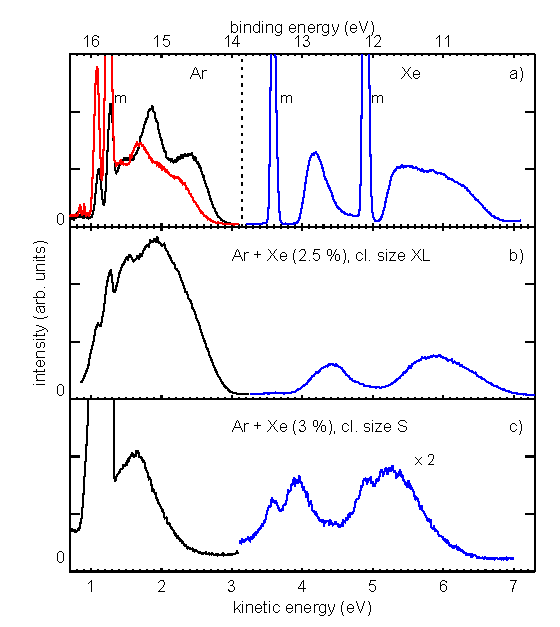
\includegraphics[width=8.5cm]{pics/figure_oval_1.pdf}
 \caption{
Outer valence photoelectron spectra of mixed Ar-Xe clusters, in comparison to the pure species. 
(a) shows the outer valence region of homogeneous Ar and Xe clusters, respectively (see text for details). 
The two lower panels show spectra of the mixed species with different mean size. 
Sharp lines marked `m' result from photoionization of uncondensed atoms into the Ar 3p$_{1/2,3/2}$ and Xe 5p$_{1/2,3/2}$ final states. 
Labels in (b) and (c) give the Xe content in the expanding gas mixture (Xe$_{\rm in}$), which is lower then the Xe content observed in the heterogeneous clusters (Xe$_{\rm cl}$). 
The photon energy was 17~eV, apart from the pure Xe cluster spectrum (60 eV).
{\color{red}{Die Stabilisierung der Xe-bulk Atome ist in den gemischten Cluster
 höher als in den gemischten Clustern. Das ist ungewöhnlich. Habt ihr hier
 verschiedene CLustergrößen?}}
}
 \label{figure:oval1}
\end{figure}


\begin{figure}[ht]
 \centering
 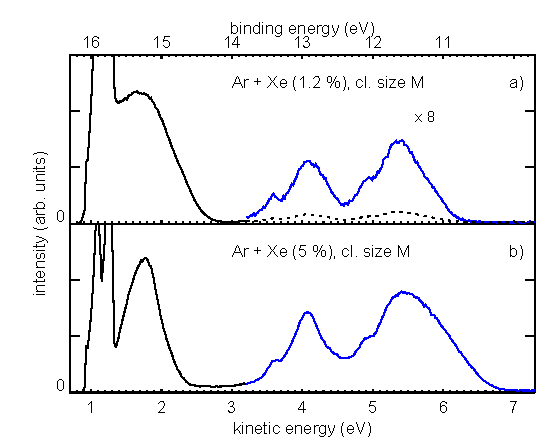
\includegraphics[width=8.5cm]{pics/figure_oval_2.pdf}
 \caption{
Outer valence photoelectron spectra of mixed Ar-Xe clusters from gas mixtures with different Xe concentration. 
For better visibility, a scaling factor is applied to the Xe part of the spectrum in (a).
See Fig.\ \ref{figure:oval1} and text for details.
}
 \label{figure:oval2}
\end{figure}

Figure \ref{figure:oval1} shows the outer valence spectra of small and large ArXe clusters, compared to clusters of the pure gases. 
Qualitatively similar spectra have been published without detailed discussion in Ref.\ \cite{lindblad}.
Differences are seen in particular for the Ar component. 
In pure Ar clusters, outer valence photoionization leads to a broad band, caused both by spin-orbit coupling and crystal field splitting. 
The relative importance of these two mechanisms remains under debate.\cite{hergenhahnprb,rolles,foerstel_arg1_2010} 
For larger clusters (e.g. $\langle N\rangle = 190$, black trace), the maximum at low binding energies becomes more pronounced, and is identified with emission from the cluster interior.\cite{hergenhahnprb,rolles}
At the particular photon energy selected here, atop of this band a sharp feature is also visible (in Figure \ref{figure:oval1} at a kinetic energy of about 1.8 eV).
For larger clusters (above $\langle N\rangle \approx 100$), over a range of photon energies of about 3 eV, its appararent binding energy changes in a way which is reminiscent to photoemission of crystalline bulk matter (`dispersion').\cite{foerstel_arg1_2010,foerstel_arg2_2011} 

Ar 3p spectra of the smaller mixed clusters (Figure \ref{figure:oval1}c, Figure \ref{figure:oval2}) show neither of these traits.
Rather, the Ar band is symmetric, less wide than in the pure clusters and at a higher binding energy.
Even for very large clusters (Figure \ref{figure:oval1}b) the asymmetry of the 3p band and the `dispersing feature' do not appear.
We characterize the spectral shape by giving a single value for the Ar 3p binding energy, and the FWHM of the feature.
Values for different expansion parameters, and for both Ar and Xe valence lines, are collected in Table\ \ref{tab:valence}.

We find experimentally that clusters we have produced have a Xe content Xe$_{\rm cl}$ between 10 and 50\,\%.
A slight decrease of the binding energy with cluster size is seen for all outer valence lines, and is attributed to a larger final state polarization energy in larger clusters. 

For further interpretation of its shape we refer to photoemission spectra of condensed Ar monolayers, measured in several settings.\cite{jacobi,jacobi2}
Spectra were reported for physisorption of Ar on two different metal single crystal substrates, and for Ar atop of a Xe spacer layer adsorbed on the metal.
While the binding energy depends on the substrate, the spectral shape is very similar in all cases. 
Most spectra were recorded for emission along the surface normal, and show a double peak split by about 0.5 eV, leading to a structure with $w$ about 1 eV.
Although the splitting is larger than the gas phase fine structure split of 0.18 eV, the pertaining states have been assigned to Ar 3p$_{1/2}$ and 3p$_{3/2}$.
A crystal field splitting of the 3p$_{3/2}$ state has been assumed to be also present, but with a smaller value of 0.1-0.2 eV, approx.\cite{jacobi2} 
The spectrum clearly changes when going to an emission angle of 40$^\circ$ with respect to the surface normal (Fig.\ 2 in Ref.\ \citenum{jacobi2}).
The higher binding energy peak significantly loses in intensity, and the spectrum is now dominated by a single peak comprising both crystal field split substates of Ar 3p$_{3/2}$, with a FWHM ($w$) of only 0.4 eV.
As our measured spectrum is comprised of contributions recorded under all emission angles with respect to the cluster surface, grazing emission will be the rule.
We therefore believe that the arguments given above make it plausible that only a single peak is observed in all our spectra.

Emission from the Xe 5p state shows a much larger fine structure splitting, which dominates the spectrum even in clusters (where other broadening mechanisms are also present). 
For the mixed clusters, the Xe band broadens and shifts towards lower binding energy for larger size clusters. 
For pure Xe clusters, an asymmetry observed in the Xe 5p$_{3/2}$ part has no counterpart in the respective spectra from the mixed clusters.
This might be caused by the difference in photon energy, as can be seen from a comparison to literature spectra (ArXe at $h\nu = 90$ eV in Ref.\ \cite{lindblad}, Xe at $h\nu = 20$ eV in Ref.\ \cite{rolles}).
For the largest clusters, the nominal size yielded from the jet parameters applied to a pure Xe expansion would correspond to clusters in which bulk atoms far outweigh those on the surface.
At least for the 5p$_{1/2}$ photoelectron line, this would be seen as a clear asymmetry towards the low binding energy side, which is not observed in our spectra.

In Figure \ref{figure:oval2}, we compare the outer valence spectra of clusters with similar expansion conditions, but different composition of the gas mixture.
A Xe-rich mixture obviously leads to clusters with more intense Xe photolines, but besides that the main change consists in a narrowing of the Ar band.
A comparison with the Ar monomer features (clipped in the Figure) also shows an increased degree of condensation for the Ar gas in the expansion.

For the smallest clusters we have produced, a plausible model is provided by calculated minimum energy structures of Ar$_N$Xe$_{38-N}$ (Fig.\ 7 in Ref.\ \cite{marques}).
We there see that for a Xe content of less than 60\,\%, core-shell systems are {\it not} formed, and although the Xe atoms tend to connect, the degree of Ar-Xe mixing is large.
While for low Xe content (approx. 10\,\%), some Ar atoms have only Ar nearest neighbours, for larger Xe content all Ar atoms seem to see both Ar and Xe nearest neighbours.
We believe this leads to the Ar 3p narrowing pointed out above.
For Figure \ref{figure:oval2}, possibly, some clusters of our ensemble already are in the core-shell regime, which would lead to an even lower 3p width.
For the largest clusters we have produced (Figure \ref{figure:oval1}b), the low binding energy of the Xe lines and the broadening of the Ar feature without appearance of the `bulk Ar'-maximum, supports formation of a Xe core covered by at least two layers of Ar.
If the scaling law size for a pure Ar expansion is taken as the lower limit for the cluster size, from the observed Xe content we arrive at clusters composed of a Xe core with four layers, covered by three layers of Ar (see Supporting Information).

Finally, comparing Figure \ref{figure:oval2} to Figure \ref{figure:oval1} reveals that much larger changes in the valence emission spectra occur by changes in
the expansion conditions than by changes of the gas mixture.
This finding is supported by the spectra shown in Ref.\ \citenum{lindblad}.
%
%
\subsection{Inner valence spectra}
%
We now focus on the Ar inner valence (3s) vacancy states. 
%
\begin{figure}[ht]
 \centering
 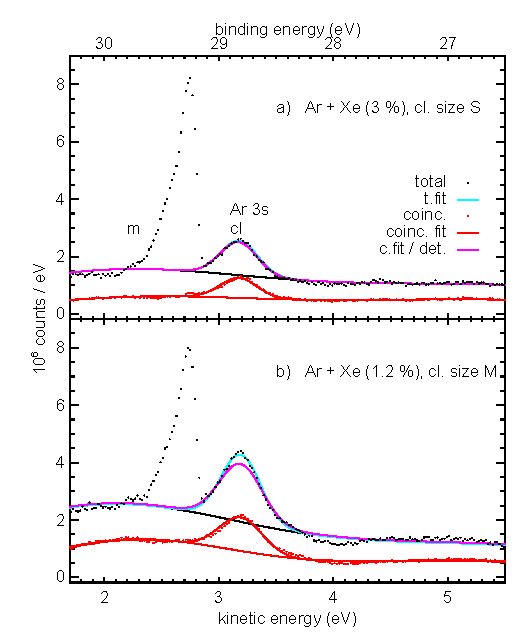
\includegraphics[width=8.8cm]{pics/figure_ival.pdf}
 \caption{
Photon excited electron spectra of mixed Ar-Xe clusters in the inner valence region.
Symbols show the Ar 3s photoline from clusters (`cl') and uncondensed Ar monomers (`m'), atop of a background resulting from inelastic intracluster scattering of outer valence photoelectrons (`excitonic satellites'\protect\cite{hergenhahn2002}).
Colored symbols result from accumulating photoelectrons only from those events, which resulted in the subsequent emission of a second electron.
Solid lines represent various least-squares fits to the data, see text for details.
A photon energy of $h\nu = 32$ eV was used.
 \label{figure:ival}
 }
\end{figure}

Figure\ \ref{figure:ival} shows the Ar part of the inner valence spectrum for representative ArXe clusters. 
The total photoelectron signal looks similar to literature spectra for pure Ar clusters.\cite{feifel,zhang} 
A low energy tail seen for the Ar 3s monomer line results from the transmission properties of the electron spectrometer, together with the strongly positive angular distribution parameter of this line.\cite{kruit}
The Ar 3s cluster line shows no splitting into bulk and surface components, different to the literature on pure clusters but in agreement with our discussion of the outer valence spectra. 
The binding energy of the cluster line has values between 28.85 and 28.70 eV for all cluster ensembles with size label S-L, and 28.67 eV for the largest clusters measured. 
A small, but systematic decrease of the binding energy is observed when the cluster size is increased. 
The value assumed in the simulations is 28.7 eV.

If we produce a spectrum only from those electrons recorded as part of a two-electron coincidence (electron pair with kinetic energies ($e_1,e_2$)) the apparent intensity drops (colored symbols in Figure \ref{figure:ival}).
This can partly be attributed to the finite detection efficiency of the spectrometer. 
Moreover, the monomer part of the Ar 3s signal completely disappears, as 3s photoionization of an uncondensed Ar atom in the gas jet cannot lead to emission of a second electron. 
Further features of these diagrams and the least squares fits shown in the Figure are discussed below.
%
%
\subsection{ICD/ETMD spectra}
%
\begin{figure}[ht]
 \centering
 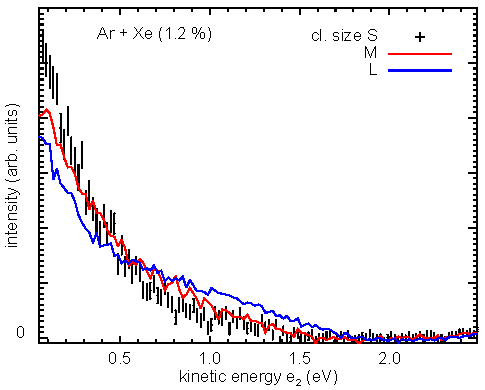
\includegraphics[width=8.5cm]{pics/figure_icd_12.pdf}
 \caption{
Energy spectrum of all coincident secondary (ICD or ETMD) electrons $e_2$ pertaining to primary electrons $e_1$ in the Ar 3s binding energy region. 
Spectra were recorded with a photon energy of $h\nu = 32$~eV. 
Black symbols with error bars show the data points for the smallest clusters measured (`S'), two larger clusters sizes are shown by the red and blue traces. 
Error bars for the latter are smaller than the ones shown and have been omitted.
For comparison, all spectra are shown area-normalized. 
}
 \label{figure:icd_12}
\end{figure}
%
%
\begin{figure}[ht]
 \centering
 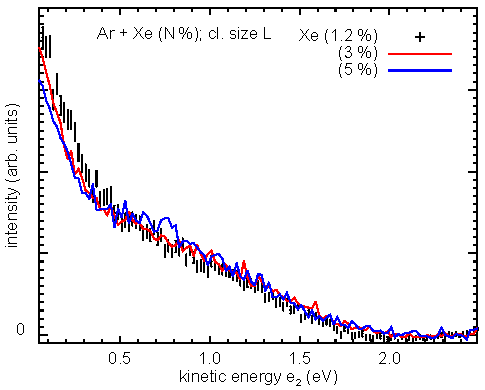
\includegraphics[width=8.5cm]{pics/figure_icd_l.pdf}
 \caption{
Energy spectrum of all coincident secondary (ICD or ETMD) electrons $e_2$ for clusters of the same size, but from gas mixtures with different Xe concentration. See Figure \protect\ref{figure:icd_12} for details.
}
 \label{figure:icd_l}
\end{figure}
%
In Figure \ref{figure:icd_12}, we show the spectra of ICD/ETMD electrons pertaining to emission of an Ar 3s cluster photoelectron. 
Due to their low kinetic energy, without use of a coincidence method they could hardly be separated from the background of inelastically scattered photoelectrons.\cite{mucke}
These, and the following figure, constitute the central experimental result of the article.
Spectra recorded at $h\nu = 34$ eV as a cross-check quantitatively agree to those shown here.
This underpins our assignment of this intensity to an autoionization process.
Further details on the data acquisition and analysis methodology, as well as the 34~eV spectra, are given in the Supporting Information.

Spectra for the three different cluster sizes in Figure \ref{figure:icd_12} are significantly different: Spectra for the larger cluster acquire more intensity in the 1-1.5 eV region and have less intensity for energies below 0.5 eV.
In contrast to that, the ICD/ETMD spectrum hardly varies when the composition of the expanding gas mixture is changed (Figure \ref{figure:icd_l}).
The full set of ICD/ETMD spectra is shown as Supporting Information.

\begin{figure}[ht]
 \centering
 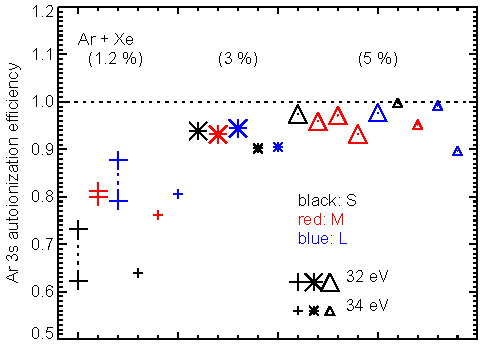
\includegraphics[width=8.5cm]{pics/figure_eff.pdf}
 \caption{
Efficiency of the decay of Ar 3s ionized states in ArXe clusters by emission of a secondary electron via ICD or ETMD. Values are arranged by Xe content of the initial gas mixture (`+' symbols: 1.2\,\%, asterisk: 3\,\%, triangle: 5\,\%). Symbol sizes indicate the photon energy (large symbols: 32 eV, small: 34 eV), and color indicates the cluster size (black symbols: S, red: M, blue: L). See text for details.
}
 \label{figure:eff}
\end{figure}
%
We now discuss which fraction of Ar 3s vacancy states relaxes via ICD or ETMD.
A method to derive this information has been established by some of us.\cite{foerstel_2013}
Briefly, we correct the intensity of the Ar 3s photoline in the coincident spectra by the detector efficiency, and divide it by the 3s intensity in the undiscriminated spectrum.
The result gives the branching ratio of decay via ICD/ETMD vs. the sum of all channels, including those not involving electron emission.
To arrive at quantitative results, we have performed least squares fits of the non-coincident and coincident $e_1$ spectra.
The fits assumed one or two Gaussian peaks, resp., atop of a background modelled by two more Gaussian curves with very large widths.
The peak pertaining to the Ar 3s cluster photoline, with the background added, is shown by the blue and red solid line in Figure \ref{figure:ival}.
Moreover, the line labelled `c.fit/det.' shows the fit to the coincident events, corrected by the detection efficiency. 
This virtually agrees with the fit to the total spectrum in Figure \ref{figure:ival}a, but not in \ref{figure:ival}b. The corresponding figure for the ICD/ETMD efficiency is at one for \ref{figure:ival}a, and significantly smaller than one for \ref{figure:ival}b.
Figure \ref{figure:eff} shows the results of this analysis.
The error in the quantity shown is mainly determined by uncertainties in the peak/background separation.
(Our choice for the background shape is shown in Figure \ref{figure:ival}.)
For the gas mixture with a Xe$_{\rm in}$ of 1.2\,\%, we therefore show results from fits using two different models.
Statistical errors are much smaller.

Within the accuracy of our experiment we found an Ar 3s autoionization efficiency which is smaller than unity for all spectra with Xe$_{\rm in}$ of 1.2\,\%, and decreases with cluster size. 
For larger Xe$_{\rm in}$, the values are compatible with unity.
